\begin{figure}[!htb]
    \begin{center}
    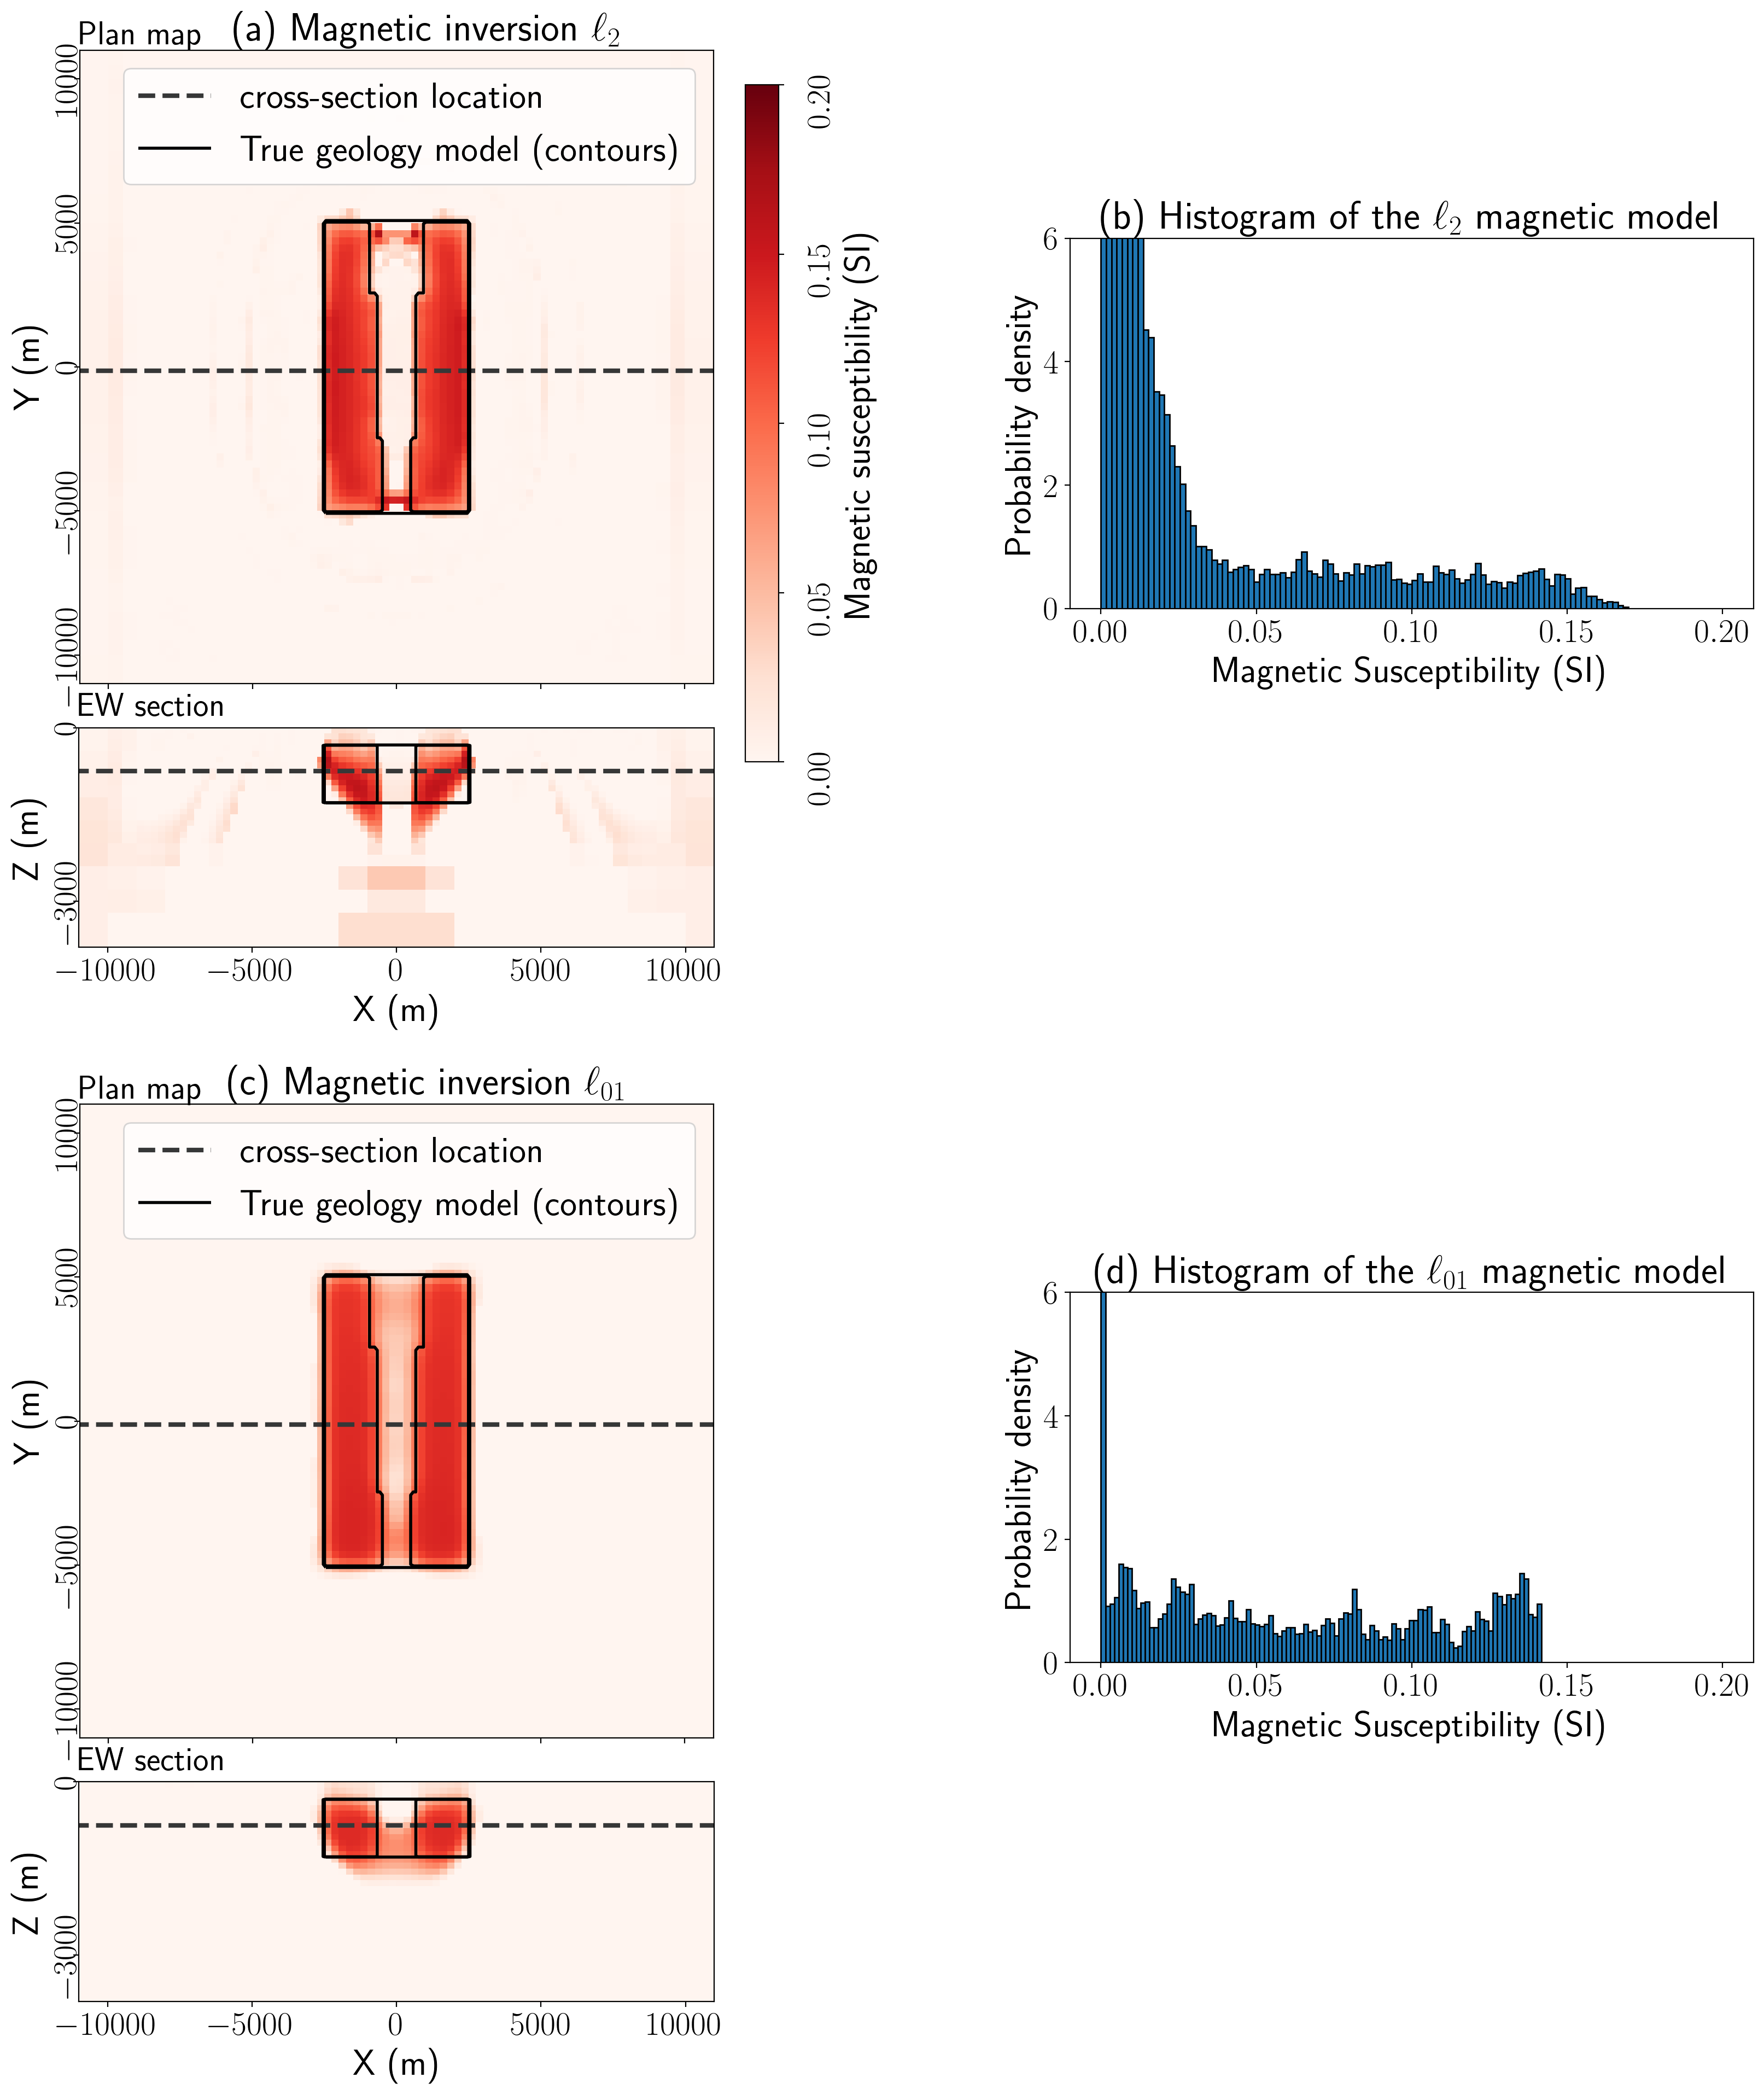
\includegraphics[width=0.7\textwidth]{figures/magnetic_l22_lpq.png}
    \end{center}
\caption{
    Models recovered using (a) an $\ell_2$ inversion of the magnetic data and (c) an $\ell_{01}$ inversion of the magnetic data. The top plot in each is a depth slice at $z=$-950m and the bottom panel shows a cross section along the line $y=0$m. Plots (b) and (d) show a histogram of the recovered susceptibility values. The histograms are normalized so that the area integrates to 1. Note that the y-limits clip the true maximum value in each.
}
\label{fig:magnetics-inversion}
\end{figure}
